\documentclass{beamer}

\usetheme{default}

\usefonttheme{structurebold}
\usepackage{helvet}
\usecolortheme{seagull}         % white on black

\usepackage[utf8]{inputenc}
\PassOptionsToPackage{hyphens}{url}\usepackage{hyperref,xspace,multicol}
\usepackage[absolute,overlay]{textpos}
\usepackage{tikz}
\usetikzlibrary{arrows,shapes,trees,shadows,positioning}
%% \usepackage{tree}
\usepackage{fancyvrb}           % for \Verb
\usepackage{ulem}               % for \sout

% Remember the position of every picture.
\tikzstyle{every picture}+=[remember picture]

\tikzset{onslide/.code args={<#1>#2}{%
  \only<#1>{\pgfkeysalso{#2}} % \pgfkeysalso doesn't change the path
}}

% Colors.
\definecolor{guixred1}{RGB}{226,0,38}  % red P
\definecolor{guixorange1}{RGB}{243,154,38}  % guixorange P
\definecolor{guixyellow}{RGB}{254,205,27}  % guixyellow P
\definecolor{guixred2}{RGB}{230,68,57}  % red S
\definecolor{guixorange2}{RGB}{236,117,40}  % guixorange S
\definecolor{guixtaupe}{RGB}{134,113,127} % guixtaupe S
\definecolor{guixgrey}{RGB}{91,94,111} % guixgrey S
\definecolor{guixblue1}{RGB}{38,109,131} % guixblue S
\definecolor{guixblue2}{RGB}{10,50,80} % guixblue S
\definecolor{guixgreen1}{RGB}{133,146,66} % guixgreen S
\definecolor{guixgreen2}{RGB}{157,193,7} % guixgreen S

\setbeamerfont{title}{size=\huge}
\setbeamerfont{frametitle}{size=\huge}

% White-on-black color theme.
\setbeamercolor{structure}{fg=guixorange1,bg=black}
\setbeamercolor{title}{fg=white,bg=black}
\setbeamercolor{date}{fg=guixorange1,bg=black}
\setbeamercolor{frametitle}{fg=white,bg=black}
\setbeamercolor{titlelike}{fg=white,bg=black}
\setbeamercolor{normal text}{fg=white,bg=black}
\setbeamercolor{alerted text}{fg=guixyellow,bg=black}
\setbeamercolor{section in toc}{fg=white,bg=black}
\setbeamercolor{section in toc shaded}{fg=white,bg=black}
\setbeamercolor{subsection in toc}{fg=guixorange1,bg=black}
\setbeamercolor{subsection in toc shaded}{fg=white,bg=black}
\setbeamercolor{subsubsection in toc}{fg=guixorange1,bg=black}
\setbeamercolor{subsubsection in toc shaded}{fg=white,bg=black}
\setbeamercolor{frametitle in toc}{fg=white,bg=black}
\setbeamercolor{local structure}{fg=guixorange1,bg=black}

\title{Reproducible and User-Controlled Package Management in HPC with GNU Guix}

\author{Ludovic Courtès (\texttt{ludovic.courtes@inria.fr})
  \\Ricardo Wurmus (\texttt{ricardo.wurmus@mdc-berlin.de})}
\date{\small{RepPar\\25 August 2015}}

\setbeamertemplate{navigation symbols}{} % remove the navigation bar

\AtBeginSection[]{
  \begin{frame}
    \frametitle{}
    \tableofcontents[currentsection, hideothersections]
  \end{frame} 
}


\AtBeginSubsection[]{
  \begin{frame}
  \frametitle{}
  \tableofcontents[currentsection, currentsubsection]
  \end{frame}
}

\begin{document}

\maketitle


% HPC system administration has to satisfy two seemingly
% contradictory demands: on one hand administrators seek stability,
% which leads to a conservative approach to software management, and
% on the other hand users demand recent tool chains and huge
% scientific software stacks.  In addition, users often need
% different versions and different variants of a given software
% package.

% To satisfy both, support teams build and install tool
% chains, libraries, and scientific software packages
% manually---multiple variants thereof---and make them available
% via ``environment modules''.

% However, HPC system users have no guarantee that they will be able
% to reproduce results at a later point in time, even on the same
% system---software may have been upgraded, removed, or recompiled
% under their feet, and they have little hope of being able to
% reproduce the same software environment elsewhere.

\begin{frame}{``Reproducibility''?}
  % Let us first define what the term "reproducibility" means when
  % applied to software and software environments in the context of
  % this talk.

  \Large{
    \begin{enumerate}
      % The most obvious and yet most elusive is reproducible software
      % builds, i.e. translating source code into bit-identical
      % binaries, across independent builds.
    \item<2-> \textbf{bit-reproducible} builds

      % Another is keeping a software *environment* constant,
      % i.e. reproducing the environment for one user on the same
      % machine across time.
    \item<3-> \textbf{isolating} a software environment from changes

      \only<4> {
        \begin{tikzpicture}[overlay]
          \node [at=(current page.center), inner sep=0mm]{
            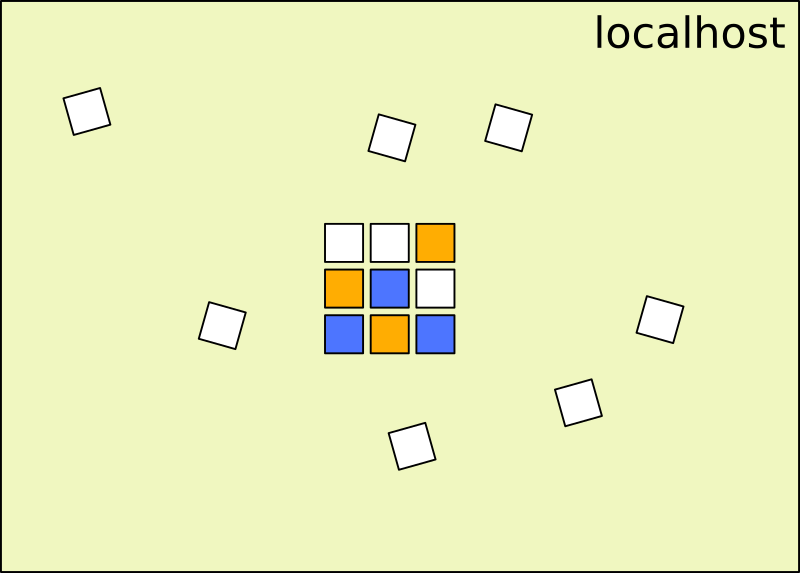
\includegraphics[width=\textwidth]{images/isolation-1}
          };
        \end{tikzpicture}
      }

      \only<5> {
        \begin{tikzpicture}[overlay]
          \node [at=(current page.center), inner sep=0mm]{
            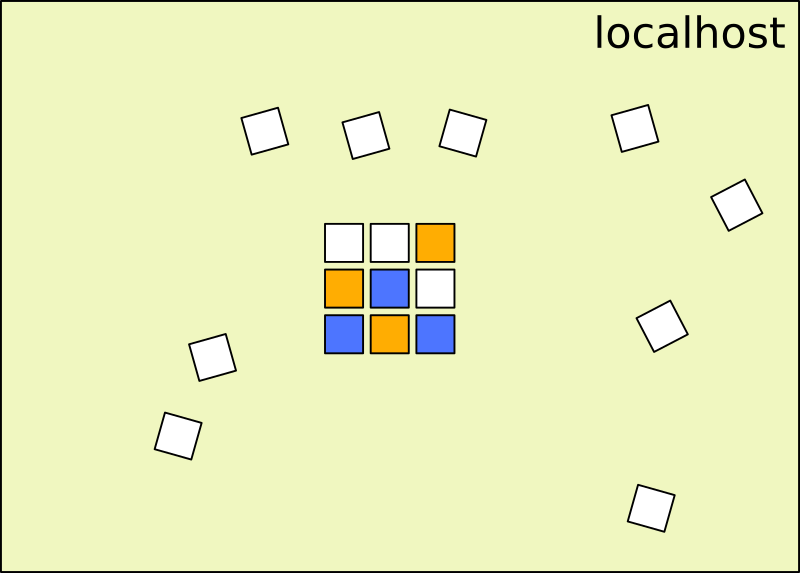
\includegraphics[width=\textwidth]{images/isolation-2}
          };
        \end{tikzpicture}
      }


      % And lastly, as an extension to the previous case, reproducing
      % an environment on a different machine and at a different point
      % in time, i.e. sharing an environment with others.
    \item<6-> \textbf{sharing} environments with others
      \only<7> {
        \begin{tikzpicture}[overlay]
          \node [at=(current page.center), inner sep=0mm]{
            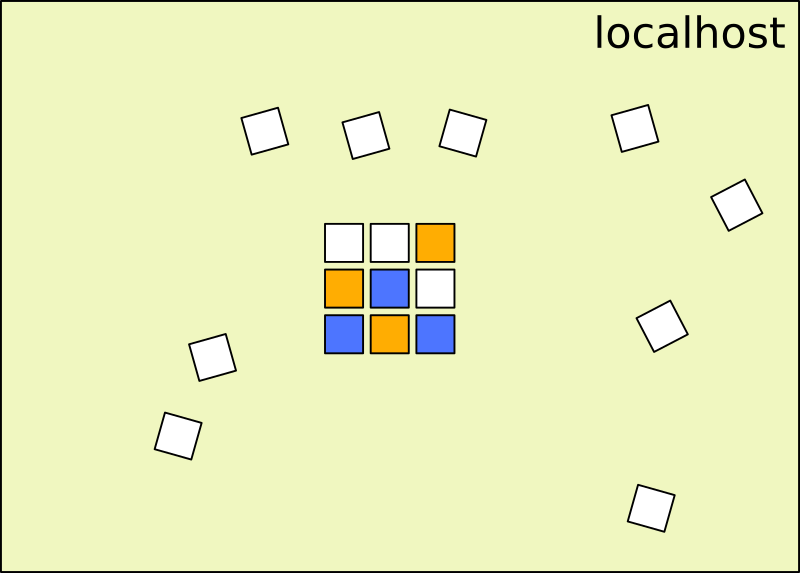
\includegraphics[width=\textwidth]{images/isolation-2}
          };
        \end{tikzpicture}
      }

      \only<8> {
        \begin{tikzpicture}[overlay]
          \node [at=(current page.center), inner sep=0mm]{
            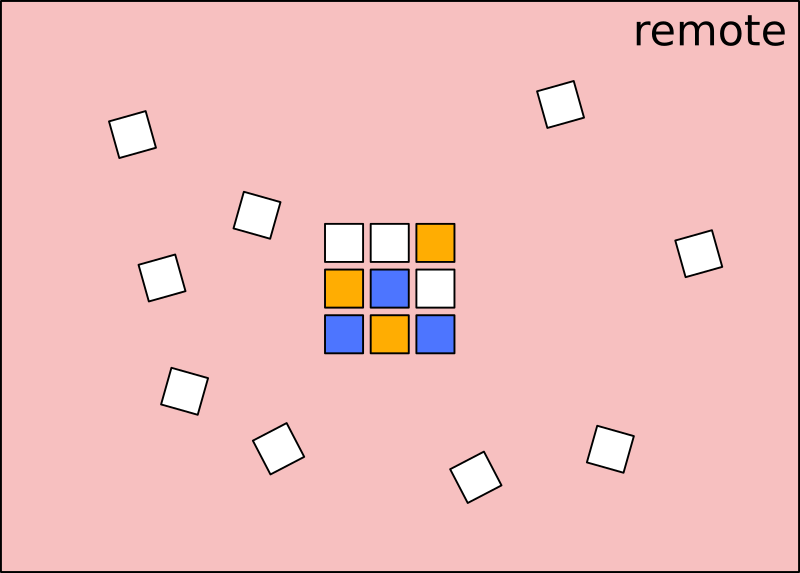
\includegraphics[width=\textwidth]{images/sharing}
          };
        \end{tikzpicture}
      }

    \end{enumerate}
  }
\end{frame}

\begin{frame}{Beyond Reproducibility}
  % To make science reproducible, it is not enough to just
  % "shrink-wrap" environments.  A necessary requirement to verifying
  % methods and results is the ability to experiment with the system.
  % The steps *after* reproducing an environment are just as
  % important as getting the environment set up in the first place.

  \Large{
    \begin{itemize}
      % The user (and nobody else) needs to have control over changes
      % the environment.  It should be easy to safely revert
      % changes and continue exploration with previous versions, to
      % make exploration cheap.
    \item<2-> \textbf{user-controlled upgrades} and roll-backs
      \only<3> {
        \begin{tikzpicture}[overlay]
          \node [at=(current page.center), inner sep=0mm]{
            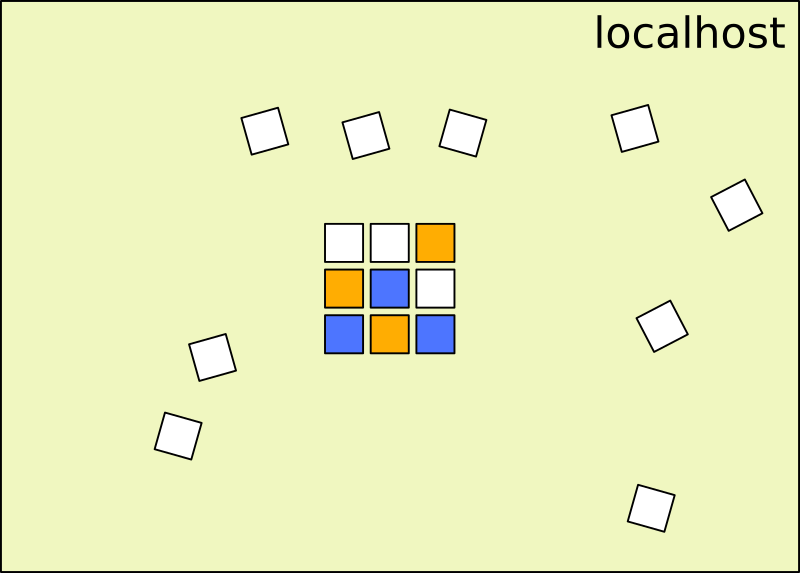
\includegraphics[width=\textwidth]{images/isolation-2}
          };
        \end{tikzpicture}
      }

      \only<4> {
        \begin{tikzpicture}[overlay]
          \node [at=(current page.center), inner sep=0mm]{
            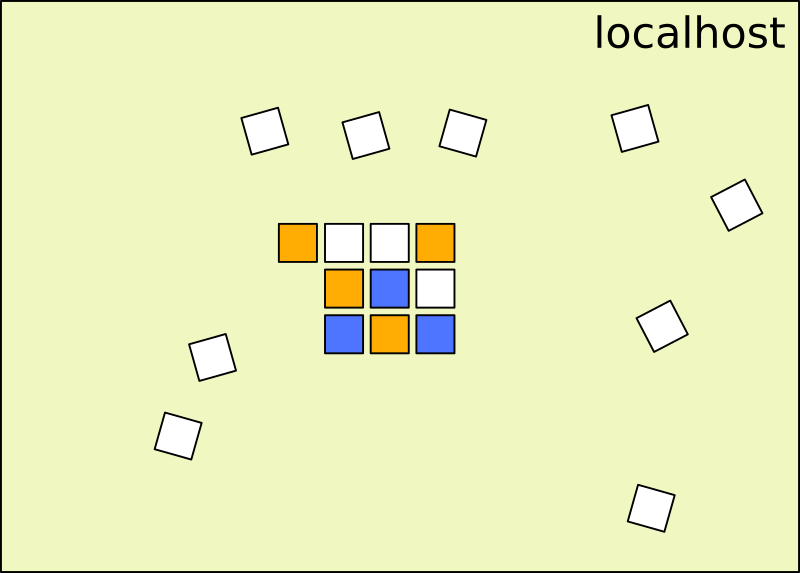
\includegraphics[width=\textwidth]{images/upgrades}
          };
        \end{tikzpicture}
      }


      % Changing *specific* parts of the software stack (e.g. a
      % dependent library, or the toolchain) must be possible to see
      % what impact they have on the result.
    \item<5-> change \textbf{specific parts} of the software stack
      \only<6> {
        \begin{tikzpicture}[overlay]
          \node [at=(current page.center), inner sep=0mm]{
            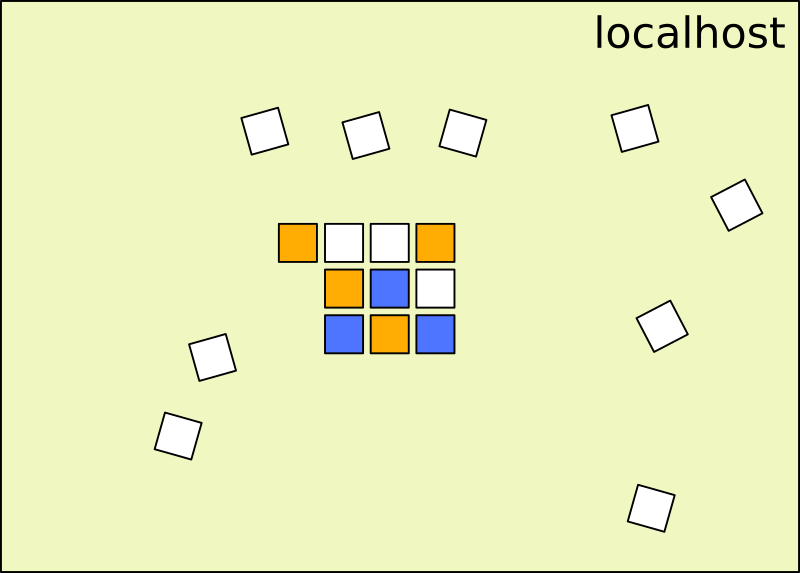
\includegraphics[width=\textwidth]{images/upgrades}
          };
        \end{tikzpicture}
      }

      \only<7> {
        \begin{tikzpicture}[overlay]
          \node [at=(current page.center), inner sep=0mm]{
            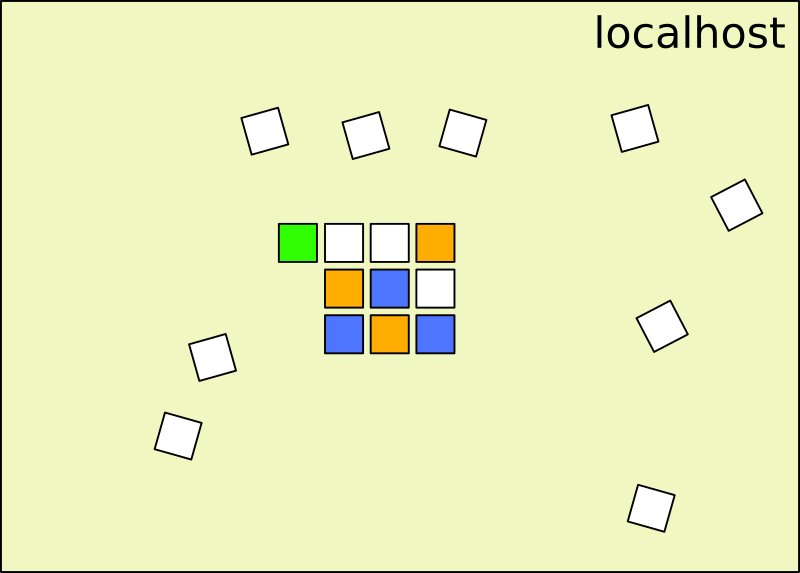
\includegraphics[width=\textwidth]{images/specific-changes}
          };
        \end{tikzpicture}
      }

      % Users should not be limited by an opaque system that cannot be
      % inspected.  It is hard to draw any scientific conclusion from
      % an experiment that relies on black boxes.
    \item<8-> \textbf{hackability}: no black boxes
    \end{itemize}
  }
\end{frame}


\begin{frame}{VMs and Docker}
  % A popular response to problems relating to deploying software
  % environments is full system virtualization or, more recently,
  % a system that makes use of containers, such as Docker.

  % This means you develop in a VM and once you're satisfied publish
  % the image; or you write and publish a Dockerfile that prescibes
  % how a base image is to be modified to reach the desired state.

  \Large{
    Pros:
    \begin{itemize}
      % It's bit-reproducible in the sense that you essentially
      % publish the bits.
    \item ``bit-reproducible''

      % Virtualization is wide-spread and is "proven technology" with
      % few surprises, making it simple for anyone to reuse an image.
    \item reproducible anywhere by anyone
    \end{itemize}
  }

  \Large{
    Problems:
    \begin{itemize}
      % VMs are heavyweight, which means they are unsuited for HPC.
      % * hardware support + KVM + in-kernel page deduplication help, but still
    \item VMs are heavyweight

      % VM images are completely opaque, binary artifacts: how can I
      % reproduce them?
      % Likewise, Dockerfiles describe steps to modify an opaque base
      % image.  How was the base image produced?  Do the binary
      % packages of the base system really correspond
      % to the source they claim to come from?

      % In both cases, inspection is difficult: we're given a pizza,
      % but not its recipe.
      % * {image of frozen pizza}
      % * {image of a very detailed recipe}
    \item binary images are opaque

      % The full system image is standalone by definition.  There is
      % no way to use the software embedded in the image *alongside*
      % other software packages I may need.

      % For example, there is no way to use, say, the library that's
      % inside the system image as-is in my own software system.

      % This encourages bad habits: modifying the image
      % state by building additional software in an ad-hoc
      % manner---we're giving up on isolation and good system
      % administration techniques.
    \item not composable
    \end{itemize}
  }
\end{frame}

%% \setbeamercolor{normal text}{fg=black,bg=guixyellow}
\begin{frame}[plain]
  \center{\huge{\textbf{functional package management}}}
  \\[2em]
  \begin{quote}
    \large{
    regarding the build \& installation process\\
    of a package as a \textbf{pure function}}
  \end{quote}
\end{frame}
%% \setbeamercolor{normal text}{fg=white,bg=black}

% FIXME: Add ``Thesis'' slide here.

\begin{frame}[fragile]
  \frametitle{From the Architecture of Nix...}
  \framesubtitle{\url{http://nixos.org/nix/}}

  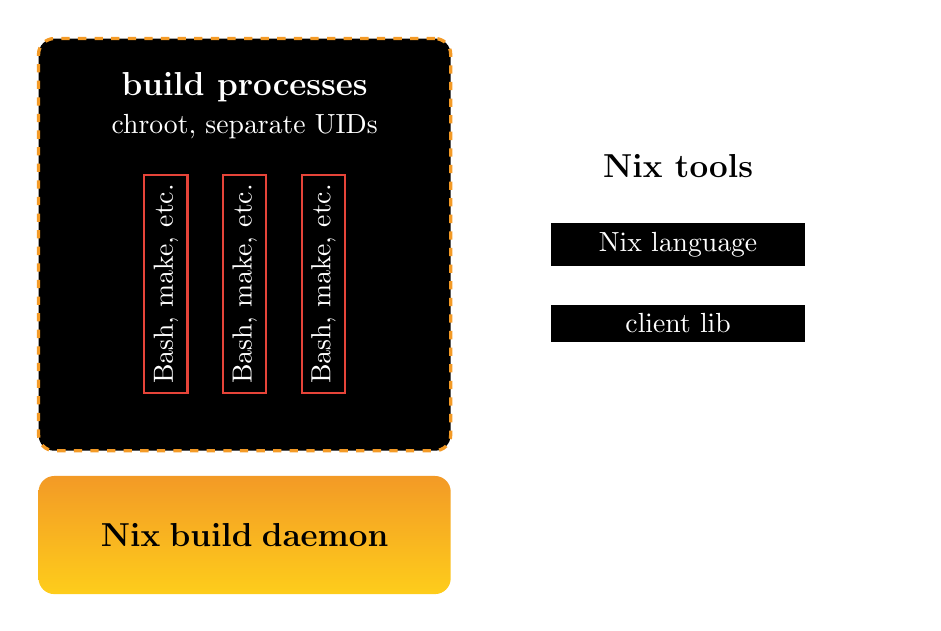
\begin{tikzpicture}[tools/.style = {
                        text width=35mm, minimum height=4cm,
                        text centered,
                        rounded corners=2mm,
                        fill=white, text=black
                      },
                      tool/.style = {
                        fill=black, text=white, text width=3cm,
                        text centered
                      },
                      daemon/.style = {
                        rectangle, text width=50mm, text centered,
                        rounded corners=2mm, minimum height=15mm,
                        top color=guixorange1,
                        bottom color=guixyellow,
                        text=black
                      },
                      builders/.style = {
                        draw=guixorange1, very thick, dashed,
                        fill=black, text=white, text width=5cm,
                        rounded corners=2mm,
                      },
                      builder/.style = {
                        draw=guixred2, thick, rectangle,
                        fill=black, text=white,
                        rotate=90
                      }]
    \matrix[row sep=3mm, column sep=1cm] {
      \node(builders)[builders, text height=5cm]{}
          node[fill=black, text=white] at (0, 2) {\large{\textbf{build processes}}}
          node[fill=black, text=white] at (0, 1.5) {chroot, separate UIDs}
          node[builder, onslide=<1-2>{black}] at (-1,-0.5) {Bash, make, etc.}
          node[builder, onslide=<1-2>{black}] at ( 0,-0.5) {Bash, make, etc.}
          node[builder, onslide=<1-2>{black}] at ( 1,-0.5) {Bash, make, etc.}; &
      \node[tools]{}
          node[fill=white, text=black] at (0, 1) {\large{\textbf{Nix tools}}}
          node[tool] at (0, 0) {Nix language}
          node(client)[tool] at (0, -1) {client lib};
      \\

      \node(daemon)[daemon]{\large{\textbf{Nix build daemon}}}; &
      &
      \\
    };
  \end{tikzpicture}

  \begin{tikzpicture}[overlay]
    \path[very thick, draw=guixorange1]<2->
      (client.south) edge [out=-90, in=0, ->] node[below, sloped]{RPCs} (daemon.east);
    \path[->, very thick, draw=guixorange1]<3->
      (daemon) edge (builders);
  \end{tikzpicture}
\end{frame}

\begin{frame}[fragile]
  \frametitle{... to the Architecture of Guix}
  \framesubtitle{\url{http://gnu.org/s/guix/}}

  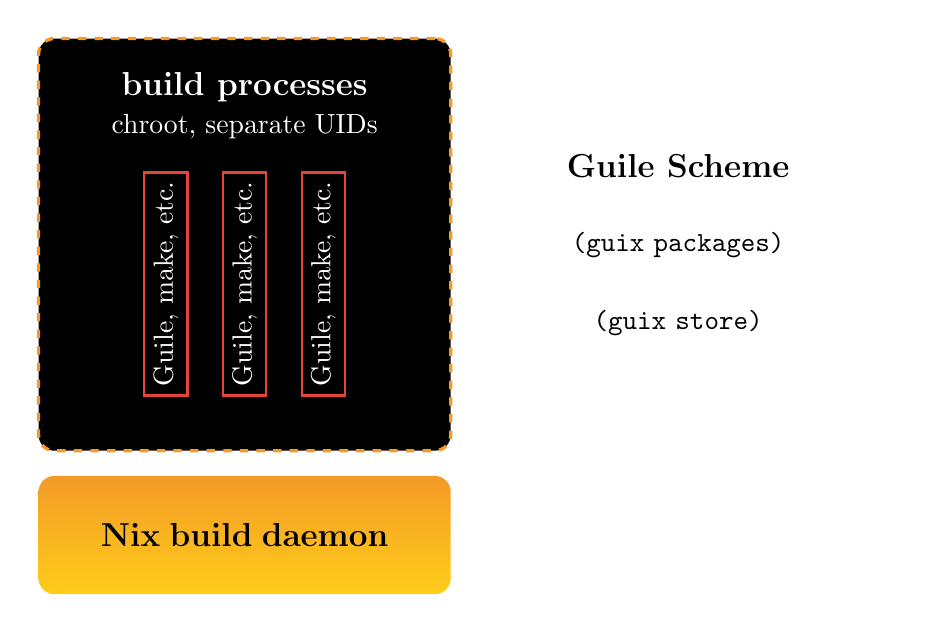
\begin{tikzpicture}[tools/.style = {
                        text width=35mm, minimum height=4cm,
                        text centered,
                        rounded corners=2mm,
                        fill=white, text=black
                      },
                      tool/.style = {
                        fill=white, text=black, text width=3cm,
                        text centered
                      },
                      daemon/.style = {
                        rectangle, text width=50mm, text centered,
                        rounded corners=2mm, minimum height=15mm,
                        top color=guixorange1,
                        bottom color=guixyellow,
                        text=black
                      },
                      builders/.style = {
                        draw=guixorange1, very thick, dashed,
                        fill=black, text=white, text width=5cm,
                        rounded corners=2mm,
                      },
                      builder/.style = {
                        draw=guixred2, thick, rectangle,
                        fill=black, text=white,
                        rotate=90
                      }]
    \matrix[row sep=3mm, column sep=1cm] {
      \node(builders)[builders, text height=5cm]{}
          node[fill=black, text=white] at (0, 2) {\large{\textbf{build processes}}}
          node[fill=black, text=white] at (0, 1.5) {chroot, separate UIDs}
          node[builder] at (-1,-0.5) {\alert{Guile}, make, etc.}
          node[builder] at ( 0,-0.5) {\alert{Guile}, make, etc.}
          node[builder] at ( 1,-0.5) {\alert{Guile}, make, etc.}; &
      \node[tools]{}
          node[fill=white, text=black] at (0, 1) {\large{\textbf{Guile Scheme}}}
          node[tool] at (0, 0) {\texttt{(guix packages)}}
          node(client)[tool] at (0, -1) {\texttt{(guix store)}};
      \\

      \node(daemon)[daemon]{\large{\textbf{Nix build daemon}}}; &
      &
      \\
    };
  \end{tikzpicture}

  \begin{tikzpicture}[overlay]
    \path[very thick, draw=guixorange1]
      (client.south) edge [out=-90, in=0, ->] node[below, sloped]{RPCs} (daemon.east);
    \path[->, very thick, draw=guixorange1]
      (daemon) edge (builders);
  \end{tikzpicture}
\end{frame}

\begin{frame}[fragile]
  \frametitle{Why Guix?}

  \Large{
    \begin{enumerate}
    \item{Scheme is a ``programmable programming language''
      \begin{itemize}
      \item we devise tailored, expressive \alert{EDSLs}
      \item can write domain-specific programs: Web UI, functions of
        packages, etc.
      \end{itemize}}
    \item \alert{general-purpose language} with compiler, debugger,
      libraries, etc.
    \item \alert{a single language} $\rightarrow$ more code reuse,
      unified environment
    \item \alert{\textbf{complete package programming interface}}
    \end{enumerate}
  }
\end{frame}

\begin{frame}[fragile]
  \frametitle{Reproducible Builds$^*$}
  \framesubtitle{$^*$ almost!}

  \begin{semiverbatim}
\$ guix build slepc
\uncover<2->{/gnu/store/\tikz[baseline]{\node[anchor=base](nixhash){\alert<2>{h2g4sf72\textrm{...}}};}-slepc-3.6.0}

\uncover<3->{\$ \alert<3>{guix gc --references /gnu/store/\textrm{...}-slepc-3.6.0}
/gnu/store/\textrm{...}-openmpi-1.8.5
/gnu/store/\textrm{...}-gfortran-4.9.3-lib
/gnu/store/\textrm{...}-superlu-4.3
/gnu/store/\textrm{...}-petsc-complex-openmpi-3.6.0
/gnu/store/\textrm{...}-glibc-2.21
\textrm{...}}
  \end{semiverbatim}

  \begin{tikzpicture}[overlay]
    \node<1>(labelnixhash) [fill=white, text=black] at (current page.center) {%
      \Large{\textbf{isolated build}: chroot, separate name spaces, etc.}
    };

    \node<2>(labelnixhash) [fill=white, text=black] at (4cm, 2cm) {%
      hash of \textbf{all} the dependencies};
    \path[->]<2>(labelnixhash.north) edge [bend left, in=180, out=-45] (nixhash.south);

    \draw<4> (-10pt, 105pt) [very thick, color=guixorange2, rounded corners=8pt]
      arc (10:-50:-50pt and 110pt);
    \node<4>[fill=white, text=black, text opacity=1, opacity=.7,
          rounded corners=2mm, inner sep=5mm]
      at (7, 2) {\textbf{\Large{(nearly) bit-identical for everyone}}};
  \end{tikzpicture}

\end{frame}


\begin{frame}[fragile]
  \frametitle{Reproducible Environments}

  \begin{semiverbatim}
\$ guix package -i gcc-toolchain coreutils sed grep
\textrm{...}


\$ eval `guix package --search-paths`
\textrm{...}


\$ guix package --manifest=my-software.scm
\textrm{...}
  \end{semiverbatim}

  \begin{tikzpicture}[overlay]
    \node[rounded corners=4, text centered,
          fill=guixorange1, text width=3cm,
          inner sep=3mm, rotate=5, opacity=.75, text opacity=1,
          drop shadow={opacity=0.5}] at (5, 4) {
            \textbf{\large{demo}}
          };
  \end{tikzpicture}
\end{frame}

\begin{frame}
  \frametitle{Experience at the Max Delbrück Center, Berlin}

  \large{
  \begin{itemize}
    \item \textbf{Guix deployed on 250-node cluster} + workstations
    \item used by \textbf{bioinformatics} researchers
    \item \textbf{50+ bioinfo packages} in use (C/C++, Python,
      etc.)
    \item replaces CentOS packages + sysadmin-managed software
  \end{itemize}
  }
\end{frame}

% FIXME: Chameleon/StarPU use case.

\begin{frame}
  \frametitle{Summary}

  \Large{
    \begin{itemize}
    \item<1-> Guix allows \alert{\textbf{cluster users}} to reproduce
      environments
    \item<2-> Guix provides \alert{\textbf{recipes}} that chefs can
      inspect \& modify
    \item<3-> \alert{\textbf{composability, transparency, and
        hackability}} of software stacks are key to reproducible
      research
    \end{itemize}
  }
\end{frame}

\begin{frame}[plain]
  \begin{tikzpicture}[overlay]
    \node [at=(current page.center), inner sep=0mm]{
      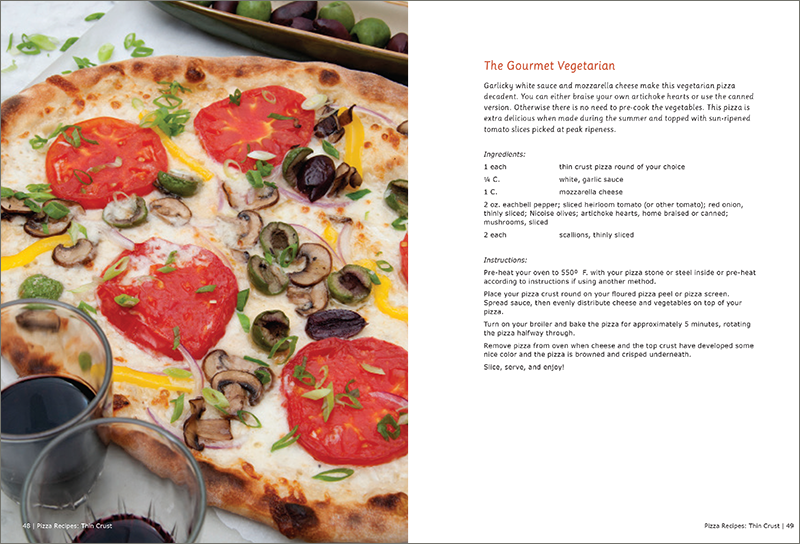
\includegraphics[height=\paperheight]{images/gourmet-vegetarian-recipe}
  };
    \node [text=black] at (current page.center) {
      \Huge{\textbf{recipes, not just pizzas}}
    };
  \end{tikzpicture}
\end{frame}

% FIXME: Add ``Thanks'' slide with tiny Guix logo.

%%%%%%%%%%%%%%%%%%%%%%%%%%%%%%%%%%%%%%%%%%%%%%%%%%%%%%%%%%%%%%%%%%%%%%%%%%%%%%
\begin{frame}{}

  \begin{textblock}{12}(2, 8)
    \tiny{
      Copyright \copyright{} 2010, 2012, 2013, 2014, 2015 Ludovic Courtès \texttt{ludo@gnu.org}.\\
      Copyright \copyright{} 2015 Ricardo Wurmus \texttt{ricardo.wurmus@mdc-berlin.de}.
      \\[3.0mm]
      GNU Guix logo, GFDL, \url{http://gnu.org/s/guix/graphics}

      Copyright of other images included in this document is held by
      their respective owners.
      \\[3.0mm]
      This work is licensed under the \alert{Creative Commons
        Attribution-Share Alike 3.0} License.  To view a copy of this
      license, visit
      \url{http://creativecommons.org/licenses/by-sa/3.0/} or send a
      letter to Creative Commons, 171 Second Street, Suite 300, San
      Francisco, California, 94105, USA.
      \\[2.0mm]
      At your option, you may instead copy, distribute and/or modify
      this document under the terms of the \alert{GNU Free Documentation
        License, Version 1.3 or any later version} published by the Free
      Software Foundation; with no Invariant Sections, no Front-Cover
      Texts, and no Back-Cover Texts.  A copy of the license is
      available at \url{http://www.gnu.org/licenses/gfdl.html}.
      \\[2.0mm]
      % Give a link to the 'Transparent Copy', as per Section 3 of the GFDL.
      The source of this document is available from
      \url{http://git.sv.gnu.org/cgit/guix/maintenance.git}.
    }
  \end{textblock}
\end{frame}

\end{document}

% Local Variables:
% coding: utf-8
% comment-start: "%"
% comment-end: ""
% ispell-local-dictionary: "american"
% compile-command: "rubber --pdf talk.tex"
% End:
